\begin{savequote}[75mm] 
Nulla facilisi. In vel sem. Morbi id urna in diam dignissim feugiat. Proin molestie tortor eu velit. Aliquam erat volutpat. Nullam ultrices, diam tempus vulputate egestas, eros pede varius leo.
\qauthor{Quoteauthor Lastname} 
\end{savequote}

\chapter{Results and discussion}
\label{chaptersix}

\section{Databases}

The most important database actions for this project are insert, retrieve and delete. We have also tested the how actions available on the file sharing services are affected by the database used. The actions of the file sharing service, in addition to the aforementioned actions, are update, retrieve publicly accessible files, retrieve files shared with user and delete all data shared by user. We have tested all actions on the Raspberry PI. We have tested these actions on the on mysql (using MyISAM storage engine) and berkelydb. Time is determined using CProfiler and in doing so, we obtain the CPU time and not the wall-clock time. The actions are executed 500 and 1000 times. This has lead us to use a relatively small file of about 521 kb. This is because the tests were conducted in an environment that had to be monitored and an increase in file size resulted in an increase in test times that made it difficult to monitor the tests. Figure \ref{fig:genericdb} shows the average operation time over 1000 runs for the labeled databases. Figure \ref{fig:filesharingdb} shows the average operation time over 1000 runs for the file sharing operations using the labeled databases.

\begin{figure}
\centering
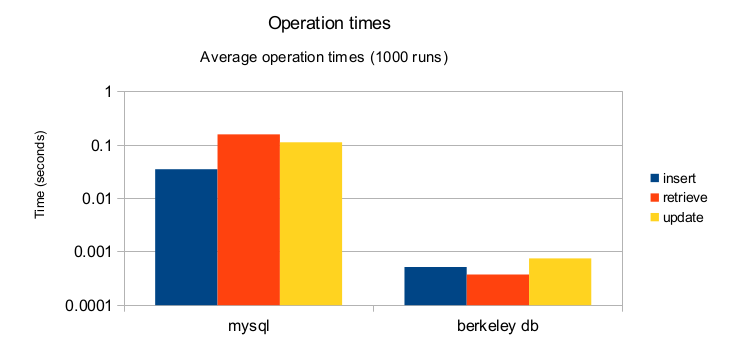
\includegraphics[scale=0.7]{figures/cprofilerdb}
\caption{}
\label{fig:genericdb}
\end{figure}

\begin{figure}
\centering
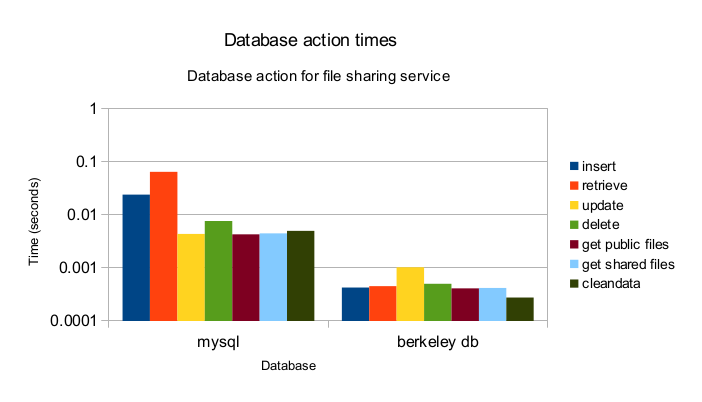
\includegraphics[scale=0.7]{figures/filesharingdb}
\caption{}
\label{fig:filesharingdb}
\end{figure}

\newpage

\section{Bandwidth}
The bandwidth decreases with an increase in distance between client and cloudlet. There are three actions from the file sharing service which are used to observe how the bandwidth changes based on distance. These actions are download, upload and viewing accessible files. Viewing accessible files is the retrieval of files which are shared with you by others and the public files. The two files which are used for this experiment are:
\begin{itemize}
\item blue.jpg - 384,5 kB
\item audio.mp3 - 2,0 MB
\end{itemize}
There are 50 iterations for each action. There are three tests conduced per action. They differ in distance. Test 1 occurs at 2.87 meters, test 2 at 4.92 meters and test 3 at 4.51 meters. The goal is to assess the bandwidth when the cloudlet is used by a human user at a specific distance. Humans do not create numerous requests within a short period of time thus flooding the cloudlet. There are periods of high bandwidth due to less activity on the network. In attempt to observe the bandwidth under such situations, the actions being studying are executed with a 50\% probability.

\begin{figure}[!h]
\centering
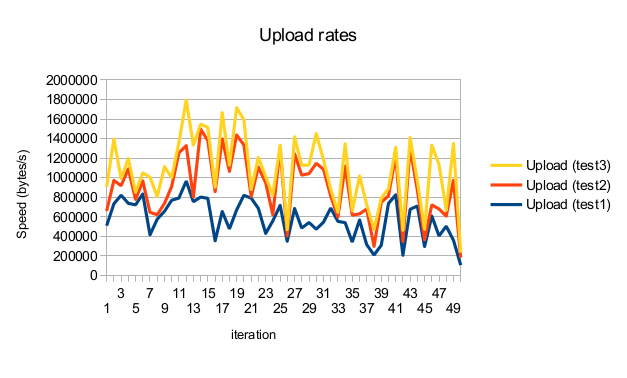
\includegraphics[scale=0.9]{figures/transferrates}
\caption{}
\end{figure}

\begin{figure}
\centering
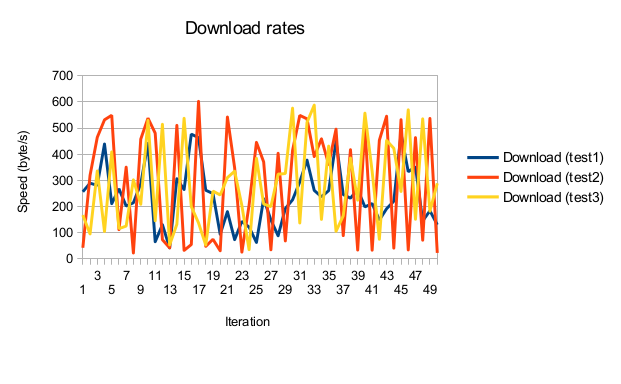
\includegraphics[scale=0.9]{figures/downloadrates}
\caption{}
\end{figure}

\begin{figure}
\centering
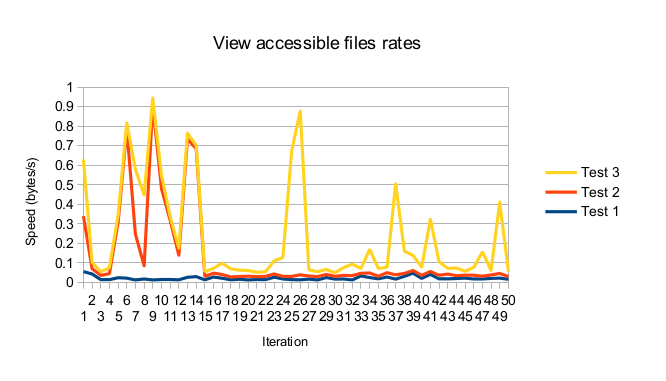
\includegraphics[scale=0.9]{figures/viewaccessiblefiles}
\end{figure}

\section{Power consumption}
The use cases presented in Chapter \ref{chapterthree} will have a large number of users connected to cloudlet at one time. This 